\documentclass{oxmathproblems}
\usepackage{graphicx}
\graphicspath{{imagenes/}} 

\course{HW 1 The Optimal Connectivity Determination in Uncertain Graphs}
\begin{document}
\vspace{-15mm}
Determining the source-destination connectivity in uncertain graphs has wide applications in real life, e.g., routing detection, information diffusion control, etc. For an uncertain graph, each edge exists independently with some probability, and the existence of each edge can be unraveled through edge testing with a certain cost. Our goal is to determine whether source s and destination t are connected or not with the minimum expected cost.
	
Given the following several kinds of uncertain graphs, please provide the corresponding optimal strategy with the minimum expected cost, and prove its optimality, respectively.
\begin{enumerate}
\item For the pyramid graph in Figure 1, each edge exists with probability $p$, and the cost of testing the existence of each edge is $1$. 
\vspace{-5mm}
\begin{figure}[htbp]
\centering
\begin{minipage}[t]{0.3\textwidth}
\centering
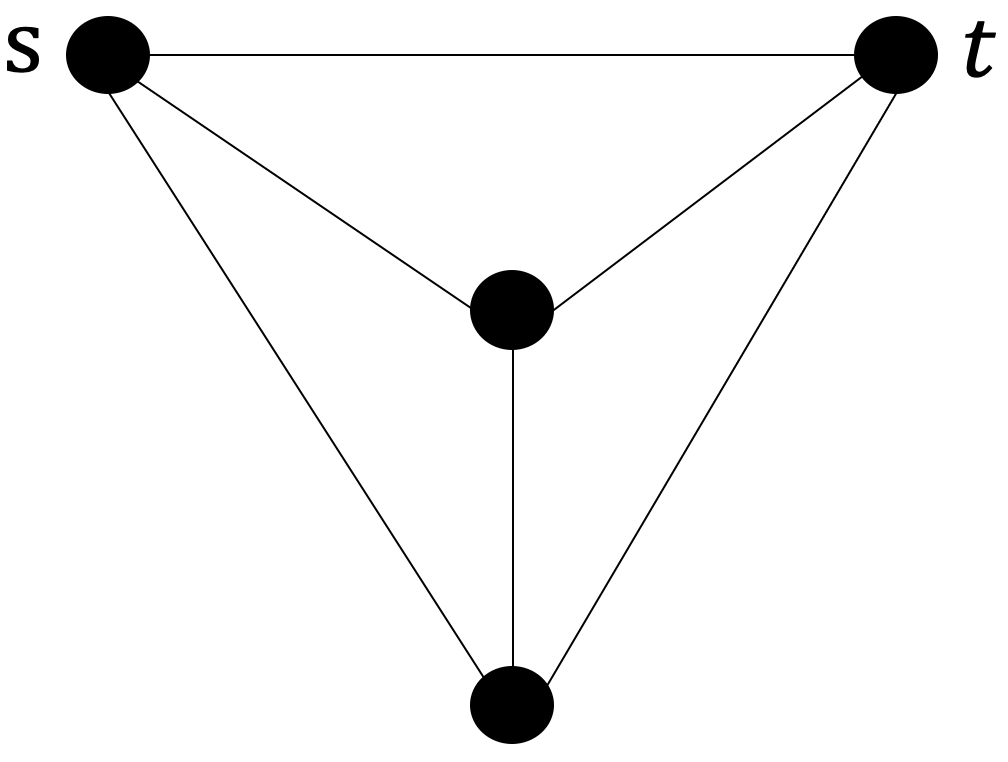
\includegraphics[width=5cm]{1.png}
\caption{Pyramid Graph}
\end{minipage}
\begin{minipage}[t]{0.48\textwidth}
\centering
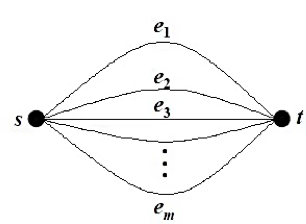
\includegraphics[width=6cm]{2.png}
\caption{Parallel Graph}
\end{minipage}
\end{figure}
\vspace{-5mm}
\item For the graph with $m$ parallel edges between nodes $s$ and $t$, edges are labeled $e_1$ through $e_m$ as shown in Figure 2. The probability that edge $e_i$ $(i=1,2,\cdots,m)$ exists is $p_i$. And the test cost of edge $e_i$ is $t_i$. 
\item  \textbf{(Optional, with additional bonus up to 2\% of your final course score.)} For the series-parallel graph consisting of $n$ parallel graph labeled $P^1_{m_1}, \cdots, P^n_{m_n}$, arranged in series. Let the $i$-th edge in the $j$-th parallel graph be represented as $e_{ij}$ $(1\leq j \leq n, 1\leq i\leq m_j)$. Edge $e_{ij}$ exists with probability $p_{ij}$ and has test cost $c_{ij}$. 
\begin{figure}[htbp]
\makebox[\textwidth][c]{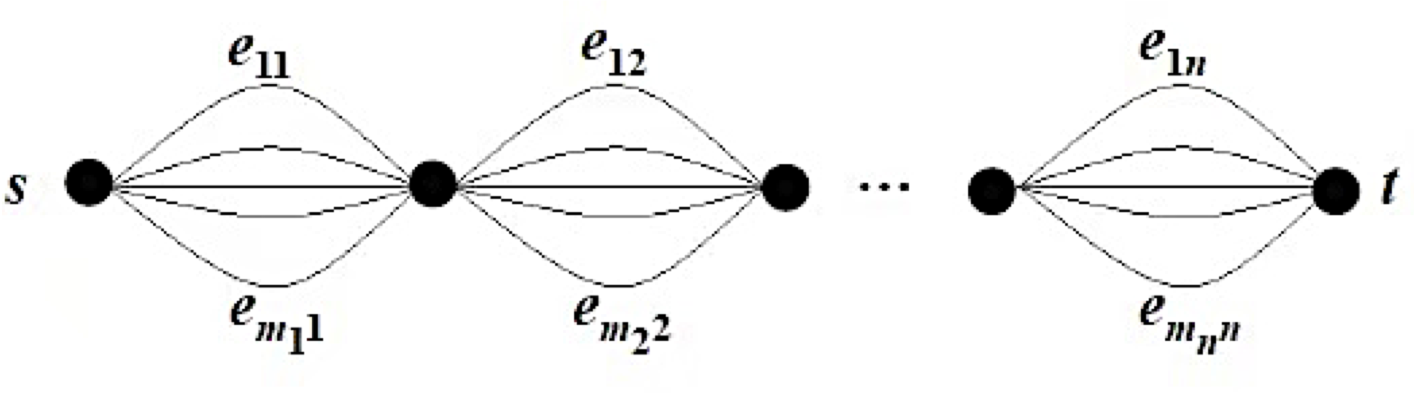
\includegraphics[width=11cm]{3.png}}
\caption{Serirs-Parallel Graph}
\end{figure}
\end{enumerate}

\begin{enumerate}
  \item {
    For simplicity we will refer to the middle node as $m$ and bottom node as $b$.

    First test the direct connection bwtween s and t, if connected, the strategy terminates. By rule 1, this choice is optimal because otherwise for s and d directly connected, an extra cost will be wasted.

    If s and d are not directly connected, a minimum cut of potential edges can be s to $m$ and $b$. By rule 2 we should not test connection between $m$ and $b$ at this moment because an extra cost can be wasted. We can test connection between either s and $m$ or s and $b$ because they are structurally equivalent. Their equivalence can be shown by stochastically coupling.

    Let's test connection between $s$ and $m$, for example. Two cases can happen.

    \begin{enumerate}
      \item If $s$ and $m$ are connected, we can view $s$ and $m$ as a cluster. By applying rule 1 again we should test the connectivity between $m$ and $t$. If connected, then strategy terminates with connected result. Otherwise, we should choose the minimum cut $b$ to $t$. If disconnected, then strategy terminates with disconnected as the result. Otherwise, cluster $\{s,m\}$ and $\{b,t\}$ remain, we should test the remaining two direct connection.
      \item If $s$ and $m$ are disconnected, the minimum cut now is $s$ and $b$. We should first test the connectivity between them. If $s$ and $b$ are disconnected, the strategy terminates with disconnected as the result. Otherwise, $s$ and $b$ forms a cluster. The only remaining potential connection is the direct connection between $b$ and $t$. We can test that to get the final result.
    \end{enumerate}

    The optimality preserves since we always apply the following rules.
    \begin{enumerate}
      \item Test the direct connection first.
      \item Pick connection in the minimum cut.
      \item Test connection with the maximum potential out edges first.
    \end{enumerate}

    Rule 3 is not actually applied since our graph is simple.

  }
  \item {
    Sort the edges in ascending order of $\frac{t_i}{p_i}$, and begin testing by choosing the edge with the lowest cost.

    We prove its optimality by constructing a inversion. After sorting, the expected cost of testing is
    \begin{equation}
      \begin{aligned}
        &p_{k_1}t_{k_1} + (1 - p_{k_1}) p_{k_2} (t_{k_1} + t_{k_2}) + \ldots + \left(\prod_{i=1}^{m-1} (1-p_{k_{i}})\right)p_{k_m}\sum_{i=1}^{m}p_{k_i} + \left(\prod_{i=1}^{m} (1-p_{k_{i}})\right)\sum_{i=1}^{m}p_{k_i} \\
        =& t_{k_1} + (1-p_{k_1})t_{k_2} + \ldots + \left(\prod_{j=1}^{m-1}(1-p_{k_j})\right)t_{k_m} \\
        =& \sum_{i=1}^{n} \left(\prod_{j=1}^{i-1}(1-p_{k_j})\right)t_{k_i} 
      \end{aligned}
    \end{equation}
    where $k_i$ are the index of edges after sorting, i.e.
    \begin{equation}
      \frac{t_{k_i}}{p_{k_i}} \le \frac{t_{k_{i+1}}}{p_{k_{i+1}}} \Rightarrow t_{k_i}p_{k_{i+1}} \le p_{k_i}t_{k_{i+1}}, \forall i
    \end{equation}

    Assume there exists an inversion between $k_i$ and $k_{i+1}$, i.e. $k_{i+1}$ is explored before $k_i$, we calculate the difference of the expected cost of testing
    \begin{equation}
      \begin{aligned}
        &C^{*} - C_{switched} \\
        = &\left(\prod_{j=1}^{i-1}(1-p_{k_j})\right)t_{k_i} + \left(\prod_{j=1}^{i}(1-p_{k_j})\right)t_{k_{i+1}} - \left(\prod_{j=1}^{i-1}(1-p_{k_j})\right)t_{k_{i+1}} \\
        & - \left(\prod_{j=1}^{i-1}(1-p_{k_j})\right)(1-p_{k_{i+1}}) t_{k_{i}} \\
        = & \left(\prod_{j=1}^{i-1}(1-p_{k_j})\right) \left(t_{k_i} + (1-p_{k_{i}})t_{k_{i+1}} - t_{k_{i+1}} - (1-p_{k_{i+1}})t_{k_i} \right) \\
        = & \left(\prod_{j=1}^{i-1}(1-p_{k_j})\right) \left(-p_{k_{i}}t_{k_{i+1}} + p_{k_{i+1}}t_{k_i} \right) \le 0
      \end{aligned}
    \end{equation}

    Thus our strategy is optimal.
  }
  \item{ An optimal strategy is to index each $s-t$ cut in each component parallel graph, in the following way:
    $$
    J_{\alpha}\left(\mathcal{P}_{m_{j}}^{j}\right)=\frac{\left(1-p_{1 j}\right)\left(1-p_{2 j}\right) \cdots\left(1-p_{m_{j} j}\right)}{t_{1 j}+\left(1-p_{1 j}\right) t_{2 j}+\ldots+\left(1-p_{1 j}\right) \cdots\left(1-p_{\left(m_{j}-1\right) j}\right) t_{m_{j} j}}
    $$
    An optimal strategy is to sample the edge e with the maximum value of $\frac{p_{e}}{t_{e}}$ on the maximum index cut.

    The optimality can be ensured with the help of the following lemma.
    
    \textbf{Lemma.} Let $\mathcal{A}=\left\{a_{1}, a_{2}, \ldots a_{m}\right\}$ be a set of edges, where edge $a_{i}$ is present with probability $p_{i}$ and incurs sampling cost $t_{i} .$ Then, the $J_{\alpha}$ index of any subset of $\mathcal{A}$ is greater than or equal to the $J_{\alpha}$ index of $\mathcal{A} .$ Equivalently, we have $J_{\alpha}\left(\mathcal{A} \backslash a_{i}\right) \geq J_{\alpha}(\mathcal{A})$

    The correctness of the lemma can be established by unfolding the definition.

    The optimality of the algorithm can be proved by induction on the number of edges in $E$.
    
    W.l.o.g we can assume that the parallel components follows an decreasing order w.r.t the index, which can be obtained by rearranging the components, and does not affect connectivity of the whole graph. We also assume that the edges in the component are sorted in ascending order of $\frac{t_i}{p_i}$.
    
    When we sample edge $e_{ij}$, it could be present or absent, resulting in two residual graphs. Both these graphs have a smaller edge set than the original graph. From the induction hypothesis, we know the optimal strategy for each of these smaller graphs. Therefore, we only need to consider the base case.

    It can be shown that the algorithm can give the minimum expected cost of the strategy for the base case. A detailed proof can be found here\footnote{Kowshik, Hemant J. Information aggregation in sensor networks, \texttt{http://hdl.handle.net/2142/24189}}.



  }
\end{enumerate}



\end{document}